\pagestyle{fancy}

\graphicspath{ {Figures/Chapter4_ThermalModel/} }

The bulk of this thesis consisted in implementing a thermal simulation code able to reproduce the thermal evolution of thin target detectors during operation.
The program implemented by M. Sapinski in 2012 for fast wire scanner simulations \parencite[][]{ref:Msapinski} was taken as a starting point. The idea started by M. Sapinski has been generalized to other types of thin target detectors, such as SEM grids, slow wire scanners and foils. Conduction cooling effects modeling has undergone a substantial update. Additionally, a (Graphical User Interface) GUI  has been implemented to facilitate the program's usage. 


\section{Introduction}

During operation, interceptive devices interact directly with the beam of particles. As was discussed in chapter \ref{ch:BeamMatterInter}, the beam of particles will deposit some energy in the detector's material. How much energy is deposited will depend on the beam energy, type of particle but also material detector and geometry. This deposited energy leads to a fast increase of the detector temperature. Depending on the beam conditions, the thermal shock suffered by the detectors can be very severe. This might affect the measured currents (Thermionic Emission), or in some cases permanently manage the detectors. 

\begin{figure}[h]
    \centering
    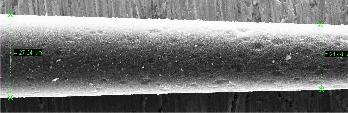
\includegraphics[width=0.60\columnwidth]{WireRadiusDeterioration/WireDamage.png}
    \caption{Carbon fiber wire scanner used at SPS in 2008.}
    \label{fig:WireRadius}
\end{figure}

At CERN, $34 \mu m$ carbon fiber wire scanners are used. Because of high brightness of proton and ion beams, the fibers are moved at high
speeds, between 1 and 6 m/s. Despite that, scanning is not possible at certain beam conditions, for instance at full LHC intensity, due to wire damage. Figure \ref{fig:WireRadius} shows a picture of a wire scanner photographed with a scanning electron microscope. This scanner was used in 2008 at CERN SPS during a systematic breakage experiment \parencite[][]{ref:Msapinski}. This picture shows how the radius of the wire was reduced due to the sublimation process after consecutively reaching high temperatures.

Another clear example of detector damage due to high temperature can be observed in Figure \ref{fig:SEMLinac4damage}. In this case, we can observe three pictures taken from a SEM grid used at LINAC4 in 2019. This grid had $40 \mu m$ gold-coated tungsten wires. Already in the first picture (left) we can observe how the gold coating was evaporated from the wires in the central part of the grid (Gold Melting Temperature is ~ 1400 K). From the images taken with the optical microscope (center), we can observe two wires glued together due to the high temperatures reached by the detector. 

\begin{figure}[h]
    \centering
    \begin{subfigure}[b]{0.42\textwidth}
        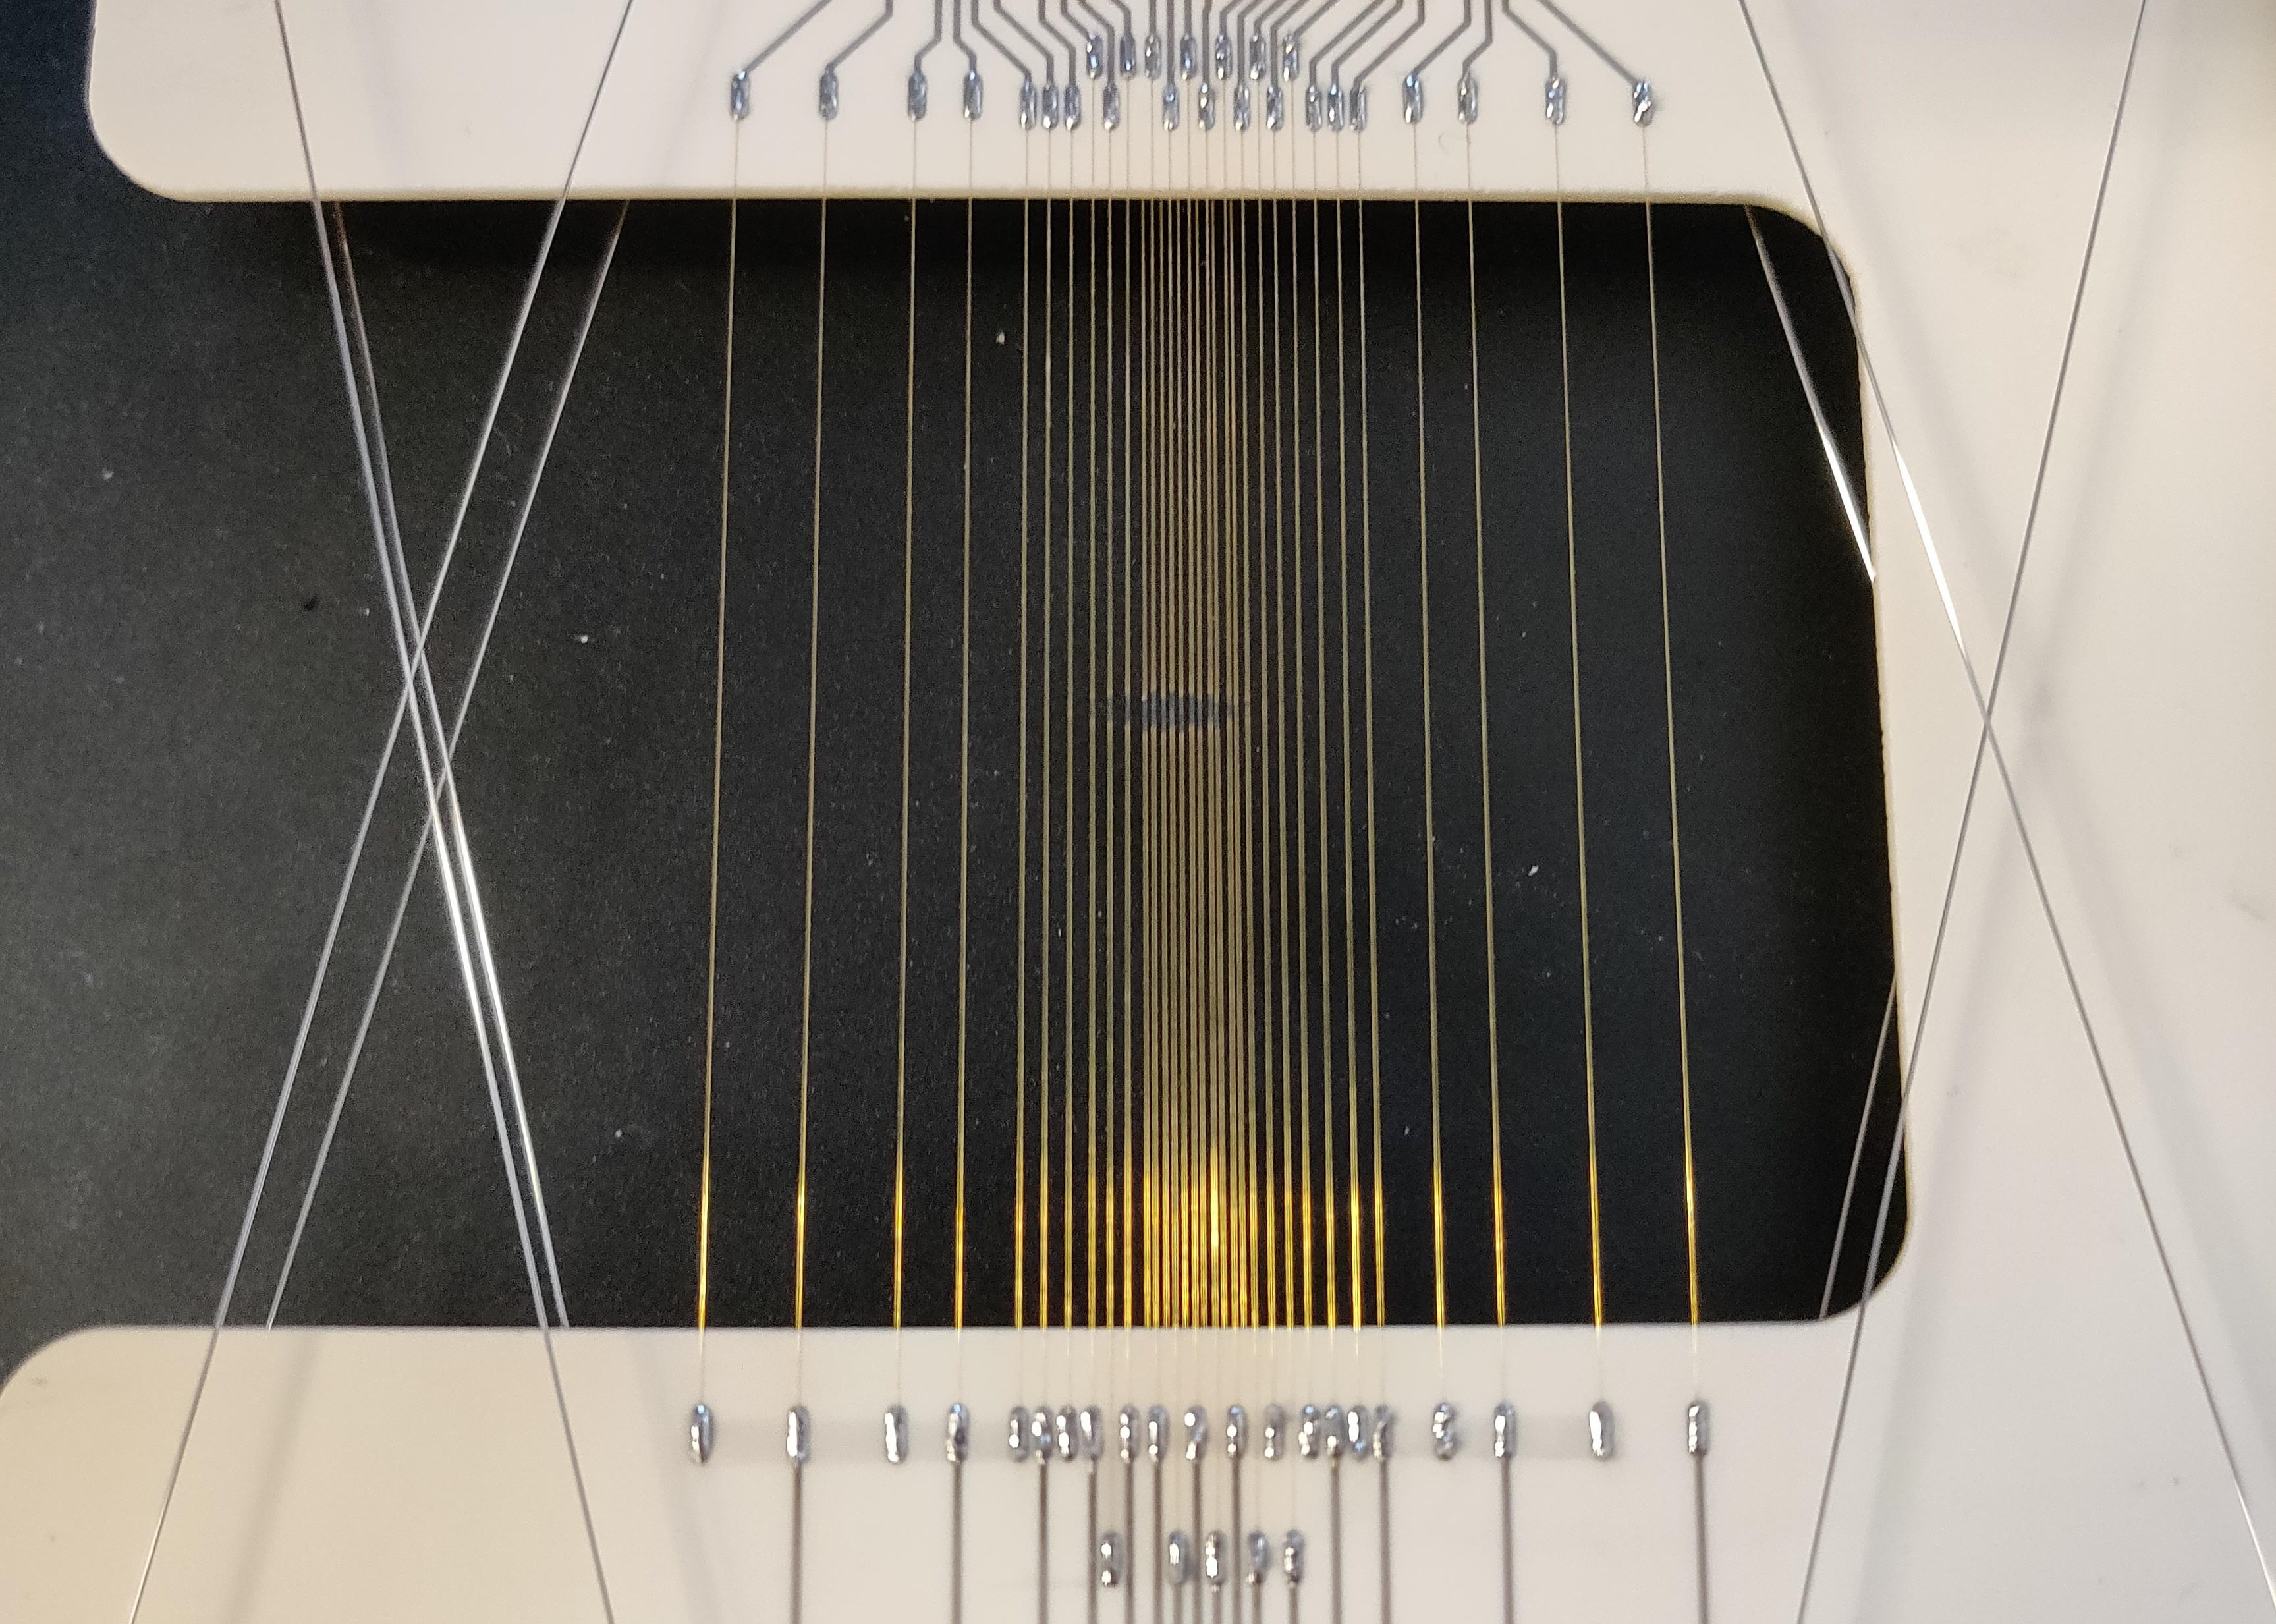
\includegraphics[width=\textwidth]{SEMgridDamage/GridDamage1.jpg}
    \end{subfigure}
    \hspace{0.5cm}
    \begin{subfigure}[b]{0.4\textwidth}
        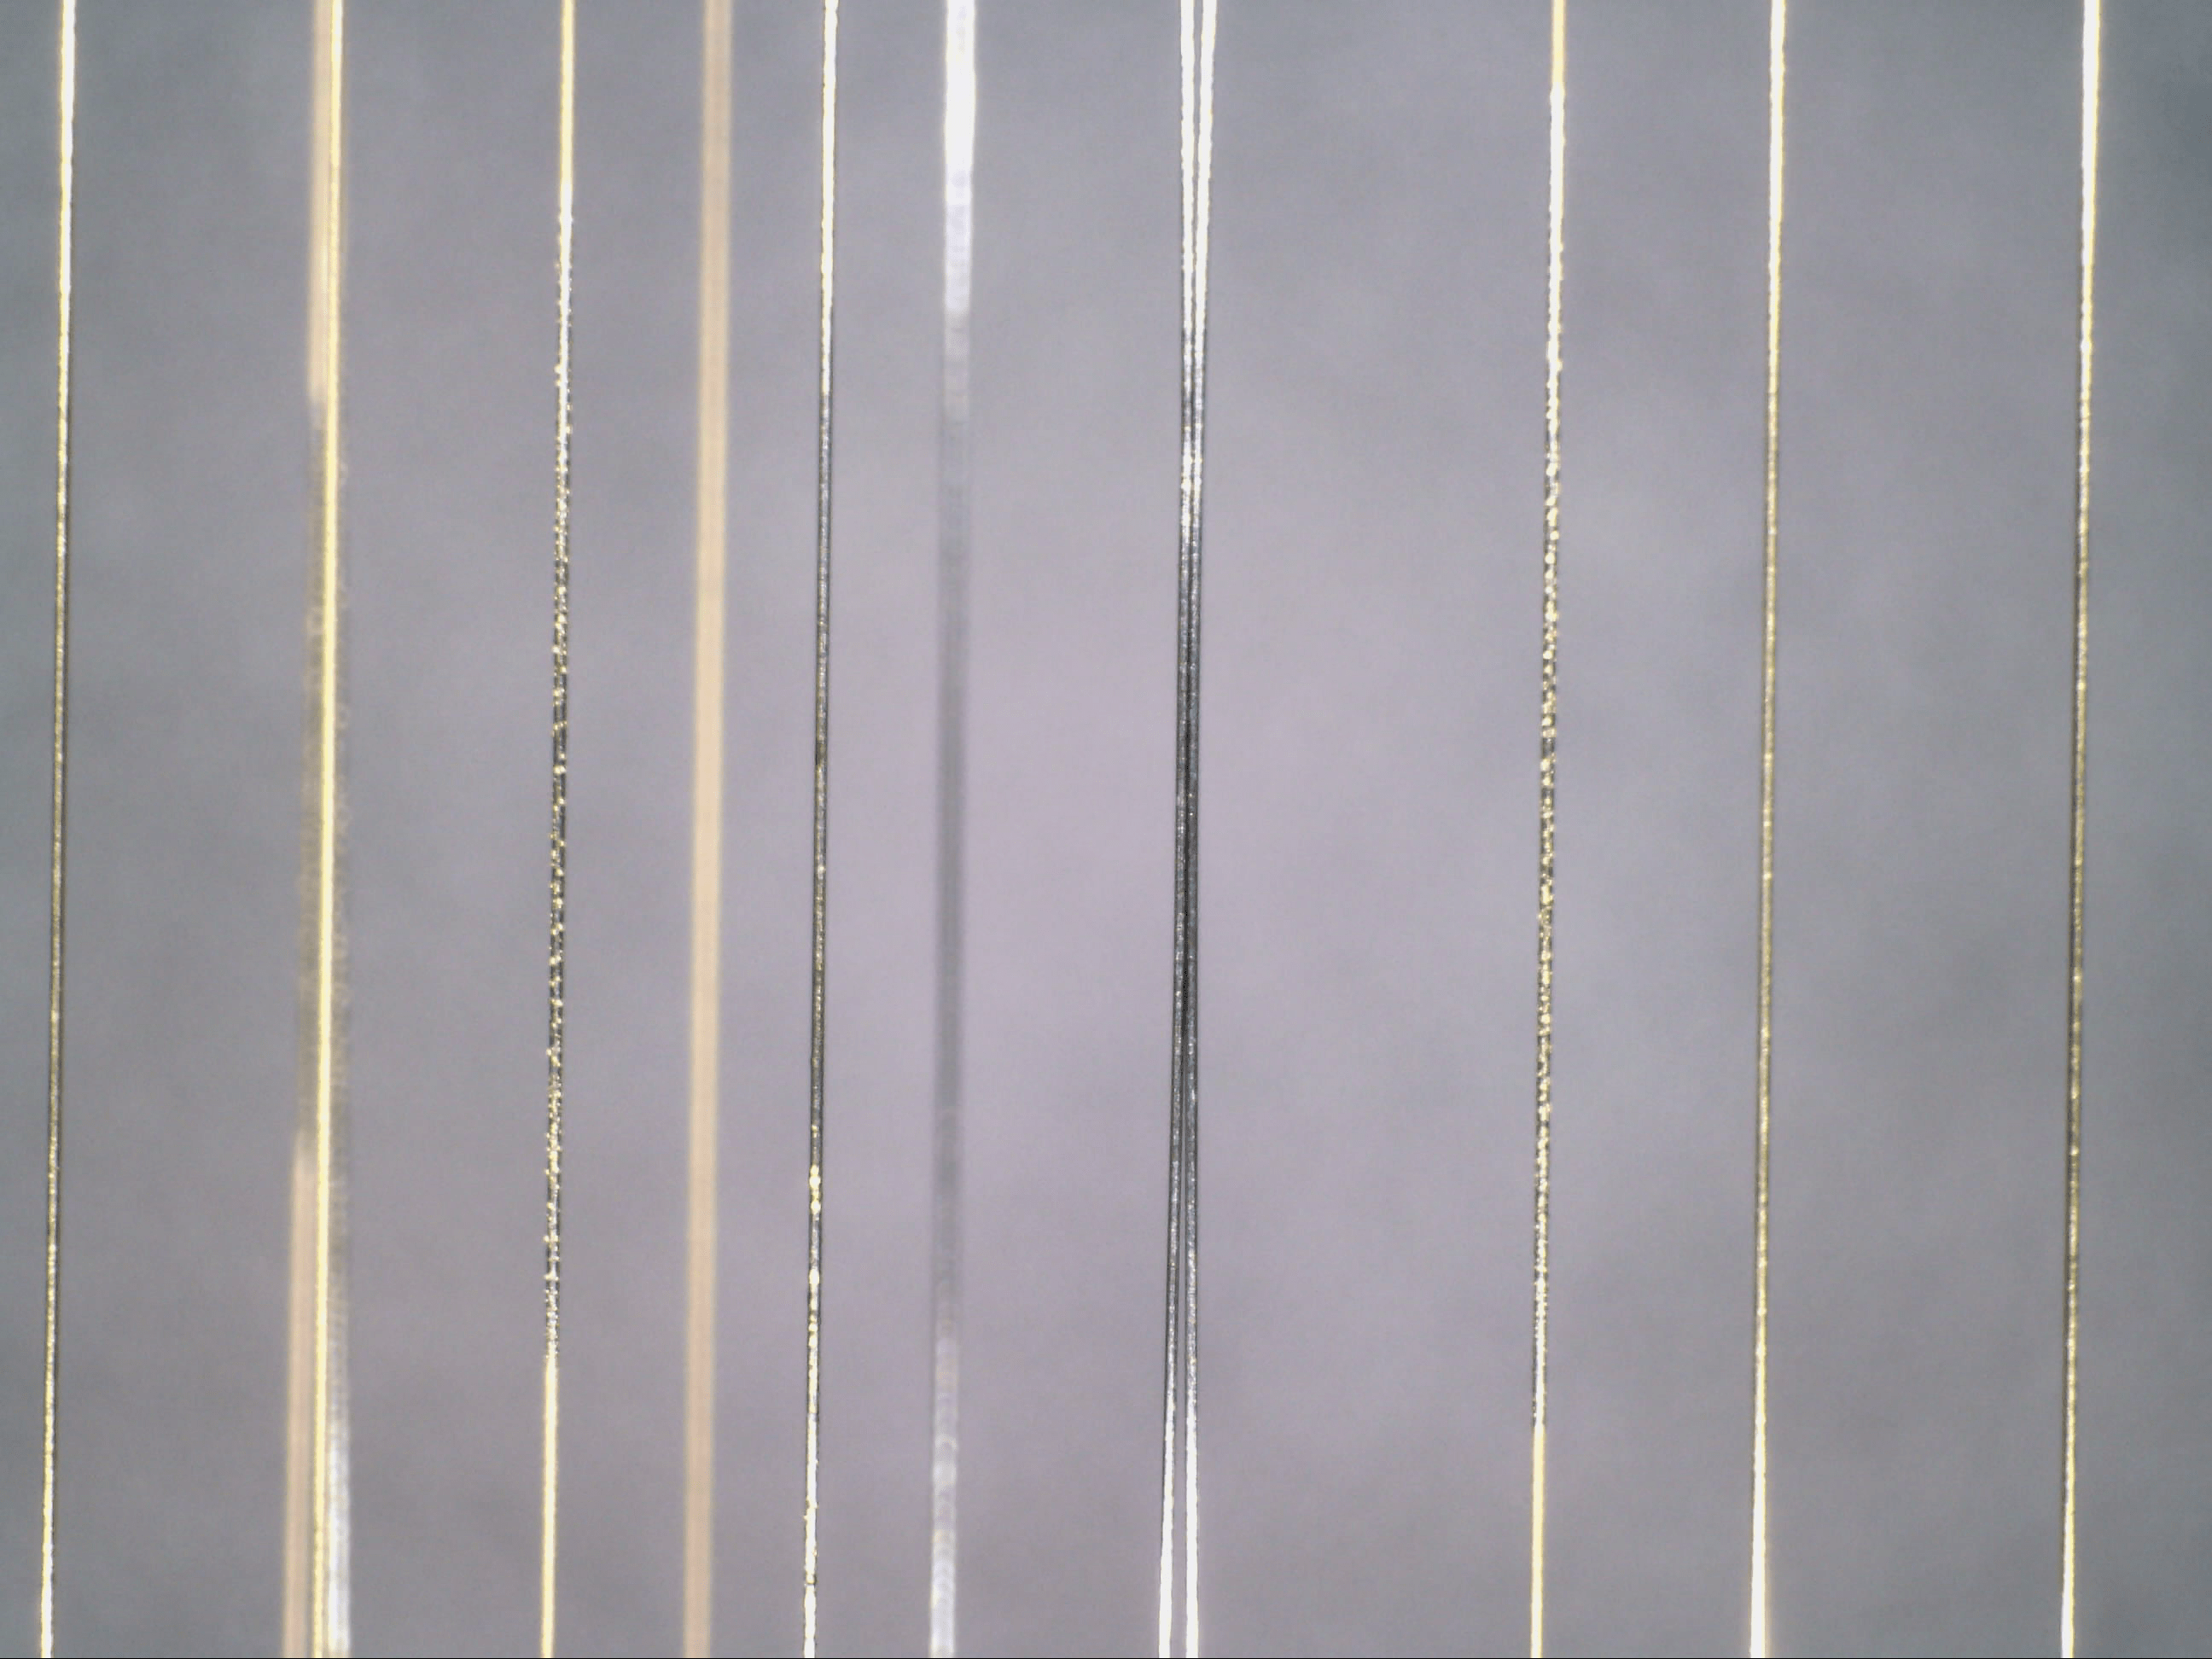
\includegraphics[width=\textwidth]{SEMgridDamage/GridDamage2.png}
    \end{subfigure}
    \caption{SEM Grid used at Linac4, in L4T Line.  }
    \label{fig:SEMLinac4damage}
\end{figure}

Figure \ref{fig:WireGluing} shows the effects wire gluing has on transverse beam profile measurements. These measurements were taken at LINAC4. In this figure, the same transverse beam profile before and after the detector damage is shown. To avoid these permanent damages, a deep understanding of the thermal evolution suffered by the detectors is necessary. 

\begin{figure}[h]
    \centering
    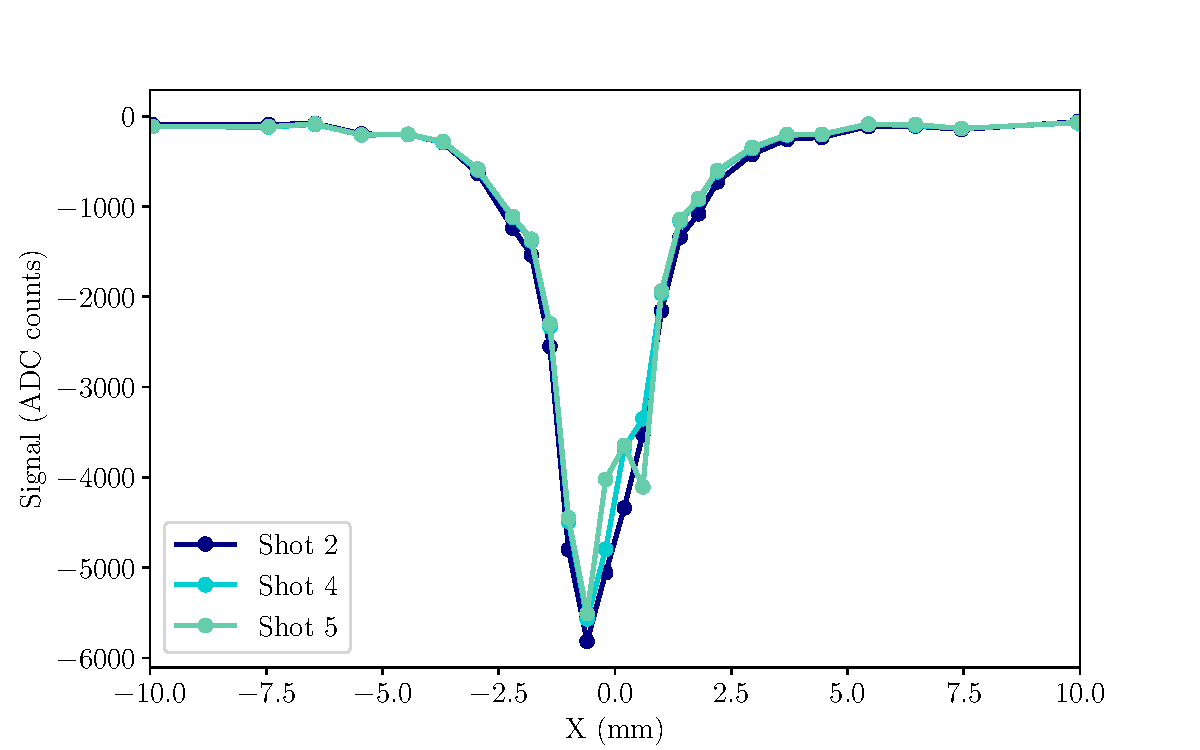
\includegraphics[width=0.60\columnwidth]{Figure_WiresGluing/WireProfile.pdf}
    \caption{Horizontal transverse beam profile of 160 MeV beam of particles at Linac4. Same beam conditions, before and after beam damage. }
    \label{fig:WireGluing}
\end{figure}



\section{The heat equation}

To understand the temperature variation of thin target detectors during operation, we need first to introduce the different processes that collaborate in this thermal evolution. In our case, the temperature variation can be described as: 

\begin{equation}
    \left(\frac{\partial T}{\partial t}\right)_{tot} = \left(\frac{\partial T}{\partial t}\right)_{Ht} - \left(\frac{\partial T}{\partial t}\right)_{Rd} - 
                 \left(\frac{\partial T}{\partial t}\right)_{Cd} - \left(\frac{\partial T}{\partial t}\right)_{Th} - \left(\frac{\partial T}{\partial t}\right)_{Sub}
    \label{eq:HeatBalance}
\end{equation}

Where the term with sub-index Ht represents the beam heating, and it is accompanied by several cooling processes such as radiative cooling (Rd), conduction cooling (Con), thermionic cooling (Th) and sublimation cooling (Sub). Because in our case this thermal model is going to be used for applications in ultra-high vacuum conditions ($10^{-6} - 10^{-9}$ (mbar)), cooling phenomena such as convection are not considered. 

To simplify the notation, the dependences of the different terms have not been included in equation \ref{eq:HeatBalance}. The temperature depends on the time (t) and on the spatial coordinates (x,y). Due to the thin target nature of the detectors, the coordinate (z) along the beam axis will not be considered. 

\subsection{Target Heating (Ht)}

Beam-induced detector heating can be traced down to two possible phenomena: 

\begin{itemize}
    \item Direct Beam Energy Deposition: It is related to nuclear and atomic interactions of the beam of particles with the material of the detector. 
    \item Indirect Electromagnetic Coupling: This is related to the energy exchange due to electromagnetic coupling between the beam of particles and the detector. 
\end{itemize}

Indirect electromagnetic coupling is a phenomenon that can be heavily mitigated by properly designing the detector geometry, and will not be covered in this work. If it is of the reader interest, a detailed description of this phenomenon can be found in \parencite[][]{ref:ElectroHeating}. One can describe the temperature variation due to direct energy deposition as follows: 

\begin{equation}
    \left(\frac{\partial T}{\partial t}\right)_{Ht} = \frac{N (x,y,t)}{V\cdot Cp(T)\cdot \rho (T)}\cdot \frac{dE}{dx}
\end{equation}

Where V, Cp(T) and $\rho (T)$ are the volume, specific heat and density of the detector's material. $dE/dx$ is the single particle energy deposition, which was explained in Chapter \ref{ch:BeamMatterInter}. N(x,y,t) refers to the surface density of beam particles reaching a point in space (x,y) at time t. This concept can be generalized to any particle distribution. However, in most cases, the beam of particles can be described as a Gaussian distribution. In that case, N(x,y) can be described as: 

\begin{equation}
    N(x,y) = \frac{N_{Tot}}{2 \pi \sigma_x \sigma_y}\cdot exp \left(
              -\frac{1}{2}\left(\frac{x-x_0}{\sigma_x}\right)^2 - \frac{1}{2}\left(\frac{y - y_0}{\sigma_y}\right)^2\right)
\end{equation}

Here $x_0$ and $y_0$ represent the coordinates of the beam centroid and $\sigma_x$ and $\sigma_y$ represent the standard deviation of the normally distributed beam of particles. $N_{tot}$ is the total number of particles (per unit time) in the particle beam. The temporal distribution can be approximated as a pulse train function. This means: 

\begin{equation}
    \begin{cases}
      N(x,y,t) = N(x,y) \mspace{30mu} if\mspace{18mu}Beam = Yes \\
      N(x,y,t) = 0 \mspace{80mu} if \mspace{18mu}Beam = No 
    \end{cases}
\end{equation}

\subsection{Radiative Cooling (Rd)}

Radiative cooling occurs due to heat transfer by thermal radiation carried by electromagnetic waves \parencite[][]{ref:RadiativeCooling}. Accelerating charged particles (electrons and protons) in the solid emit photons (or electromagnetic waves) that carry energy with them. In vacuum,  or in materials that allow the transmission of electromagnetic waves, radiation cooling might be of great importance. 

Radiative cooling is a surface effect, and it depends on the surface characteristics and its temperature.  The net temperature variation from a surface S at a temperature T to a surrounding large enclosure at temperature $T_0$ can be described by Stephan-Boltzman's law as follows: 

\begin{equation}
    \left( \frac{\partial T}{dt} \right)_{Rad} = \frac{S\cdot \sigma_{SB}\cdot \epsilon(T)\cdot \left(T(x,y,t)^4 - T_0^4\right)}{Cp(T)\cdot V \cdot \rho(T)}
\end{equation}

Where $\sigma_{Sb}$ is the Stephan-Boltzmann constant and $\epsilon$ is the emissivity of the material. Emissivity is a measure of the efficiency with which a surface emits thermal energy and it is defined as the ratio of the energy radiated from a material's surface to that radiated from a perfect emitter, known as black-body. A more detailed description of the emissivity can be found in chapter \ref{ch:EmissivityMeas}. 

\subsection{Conduction Cooling (Cd)}

Thermal conduction in solids or static fluids \parencite[][]{ref:ConductionCooling} occurs as soon as a spatial temperature gradient exists. The carriers of the energy transfer can be molecules, atoms, electrons and phonons. The rate of change due to conduction can be described by Fourier's equation as follows: 

\begin{equation}
    \left( \frac{\partial T}{\partial t} \right)_{Cond} = \alpha (T) \left( \frac{\partial^2 T}{\partial x^2} + \frac{\partial^2 T}{\partial y^2} \right)
\end{equation}

$\alpha(T)$ is called the thermal diffusivity of the medium and it measures the rate of heat transfer in a material from the hot end to the cold end. It has SI units of $m^2 /s$. It can be calculated as follows: 

\begin{equation}
    \alpha(T) = \frac{k(T)}{\rho(T)Cp(T)}
\end{equation}

Where k(T) is defined as the thermal conductivity of the material (W/mK), which is the measure of the capability of the material to conduct heat. In general, metals have high thermal conductivity and gases have low thermal conductivity. 

\subsection{Thermionic Cooling (Th)}

Thermionic emission was introduced in chapter \ref{ch:CurrentModeling}. As was said before, thermionic emission is a process by which free electrons are emitted from the surface of a metal when they gain enough thermal energy to overcome the work function. These thermionic electrons take with them some energy, and this contributes to the thermal cooling \parencite[][]{ref:ThermoCooling}. The temperature variation due to thermionic emission can be described as: 

\begin{equation}
    \left(\frac{\partial T}{\partial t}\right)_{Th} = S\cdot \left( \phi +2K_B T\right)\cdot \frac{J_{Th}(T)}{C_p(T)\cdot V \cdot \rho(T)}
\end{equation}

Where $\phi$ is the work function of the material. $K_B$ is Boltzmann constant. $J_{th} (T)$ was described in section \ref{sec:ThermoCurrent} can be written as: 

\begin{equation}
    J_{th} (T) = A_R \cdot T^2\cdot exp\left(-\frac{\phi}{K_B T}\right)
\end{equation}

\subsection{Sublimation Cooling (Sub)}

Sublimation is the process of changing a solid into a gas without passing through the liquid phase. To sublimate a substance, certain energy must be provided. We will call this energy $H_{sub}$, and it must be sufficient to break the intermolecular forces holding the solid together. Usually it is expressed in (KJ/mol) and can be found in the literature. Similar to the thermionic case, the newly formed gas molecules will escape the material, and the energy given to them for transforming their estate contributes to the overall cooling of the detector \parencite[][]{ref:SublimationCooling}. This sublimation cooling can be written as: 

\begin{equation}
    \left(\frac{\partial T}{\partial t}\right)_{Sub} = H_{sub}\cdot n(T)
\end{equation}

n(T) is the material sublimation rate. Following the same procedure as \parencite[][]{ref:SubRate}, one can determine an upper limit of this sublimation rate. For that one needs to assume the following: 

\begin{itemize}
    \item No atoms leaving the boundary layer return to the hot surface. 
    \item A thin boundary layer over the hot material surface is at equilibrium with the substance sublimation pressure ($P_{vap}$) for temperature $T_{vap}$. 
    \item This thin layer of gas is considered to be an ideal gas. 
\end{itemize}

With these approximations, the amount of sublimated material per unit of time can be expressed as: 

\begin{equation}
    d_{sub} = \frac{1}{2}v_{vap}\cdot \rho_{vap} \cdot \rho_{c}
    \label{eq:SubMaterial}
\end{equation}

$v_{vap}$ is the velocity of the vapor particles. From an ideal gas theory, we know that the average velocity of gas particles in a hemisphere can be described as follows: 

\begin{equation}
    v_{vap} = \frac{1}{2}\cdot \sqrt{\frac{8k_B T_{vap}}{m \pi}}
\end{equation}

Where m is the mass of the material particle. In equation \ref{eq:SubMaterial}, $\rho_{vap}$ refers to the vapor density in the equilibrium layer and can be expressed using the formula: 

\begin{equation}
    rho_{vap} = \frac{m_{mol} T_{std}}{V_{mol} P_{atm}}\cdot \frac{P_{vap}(T_{vap})}{T_{vap}}
\end{equation}

Where $P_{atm}$ is the atmospheric pressure ($10^5$ Pa), $V_{mol} = 22.4$ $dm^3$is the molar volume of an ideal gas at the standard temperature $T_{std} = 273$ K. The vapor pressure highly depends on the maximum temperature of the material, and thus, the total amount of sublimated material will highly depend on the temperatures reached. 

\section{Numerical Approximation to the heat equation.}

Putting together all the concepts from the previous section, we can re-write equation \ref{eq:HeatBalance} as follows: 

\begin{multline}
    \left(\frac{\partial T}{\partial t}\right)_{Tot} = 
    \frac{N(x,y,t)}{V\cdot Cp(T) \cdot \rho (T) }\cdot \frac{dE}{dx} \\
    - \frac{S\cdot \sigma_{SB}\cdot \epsilon(T)\cdot \left(T^4 - T_0^4\right)}{Cp(T)\cdot V \cdot \rho(T)} 
        -\alpha (T) \left( \frac{\partial^2 T}{\partial x^2} + \frac{\partial^2 T}{\partial y^2} \right)  \\
        - S\cdot \left( \phi +2K_B T\right)\cdot \frac{J_{Th}(T)}{C_p(T)\cdot V \cdot \rho(T)} - H_{sub} \cdot n(T)
    \label{eq:ExplicitHeatEq}
\end{multline}

This is an evolutionary, non-linear, second order, partial differential equation (PDE). In this work, this equation is treated numerically. The subject of PDEs and how to solve them is very broad. An enormous number of different numerical techniques to solve non-linear or quasi-linear PDEs exist. For an outstanding introduction to this world, I recommend the reader to check \parencite[][]{ref:NumericalMethodBook}, where a small number of tools are introduced forming a solid basis for the understanding of the subject. 

In this document, we will focus on the classical theory of finite differences. The main idea in the calculus of finite differences is to replace derivatives with linear combinations of discrete function values. The word discrete means that the numerical solution is known only at a finite number of points (or nodes) in the physical domain. Figure \ref{fig:SpaceDiscret} shows an example of the spatial discretization of a homogeneous body. 

\begin{figure}[h]
    \centering
    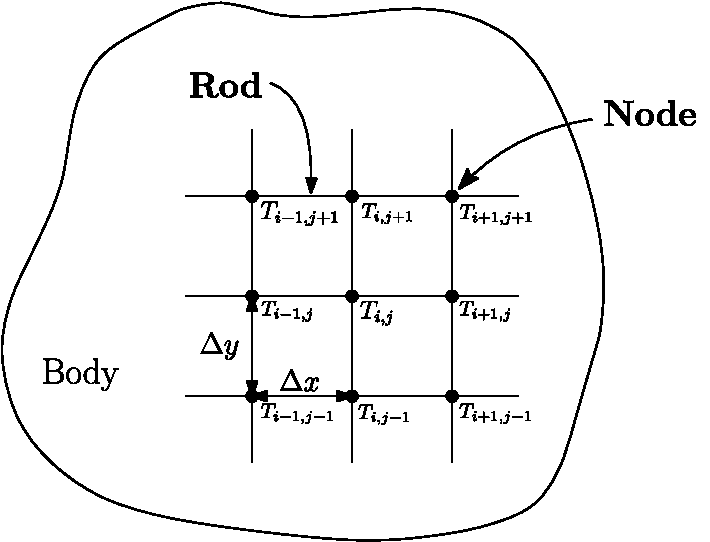
\includegraphics[width=0.5\columnwidth]{SpaceDiscretization/SpaceDiscretization.pdf}
    \caption{Space discretization of a homogeneous body.}
    \label{fig:SpaceDiscret}
\end{figure}

The parameters $\Delta x$ and $\Delta y$ indicate the local distance between adjacent points in space, and in our case, they are considered to be uniform throughout the mesh. Increasing the number of nodes in the mesh (reducing $\Delta x , \Delta y$) increases the resolution and the accuracy of the numerical solution. However, it increases computational costs.

Every node in the grid has a temperature and can exchange heat with its neighbors through a heat conducting rod. The sub-indexes i, j are used to refer to nodes in the physical space.  $T_{i,j}$ refers to the temperature in the position $x_i , y_j$.

Because the temperature of the system changes a function of time, the numerical solution of the PDE requires also time discretization. Figure \ref{fig:TimeDiscret} shows a schematic representation of the time discretization of a strip of material. The time nodes are referred to with the super-index m, so that $T^{m}$ corresponds to the temperature at the time instant  $t^m$.  $\Delta t$ refers to the difference between time nodes. This distance was also considered to be equidistant, however, two different time constants were considered, one for the heating time ($\Delta {t}_{heat}$) and one for the cooling period ($\Delta t_{Coold}$). In most applications, the beam of particles is pulsed, and the beam pulse length is much shorter than the period without beam. 

\begin{figure}[h]
    \centering
    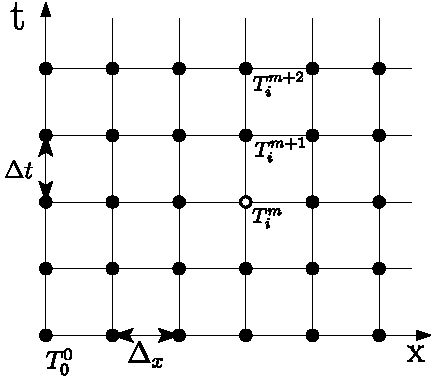
\includegraphics[width=0.4\columnwidth]{TimeDiscretization/TimeDiscret.pdf}
    \caption{Time discretization of the material rod.}
    \label{fig:TimeDiscret}
\end{figure}

\section{Finite Differences Schemes}
\label{sec:FD}

Working with the full heat equation (eq. \ref{eq:ExplicitHeatEq}) can result in a very cumbersome notation. 
The one-dimensional case of a thin rod will be considered, with only radiative and conduction cooling will be considered in this section. The concepts can be easily extrapolated to the full 2D case and some hints on that will be given in the following sections.  The simplified equation that we will treat here is: 

\begin{equation}
    \frac{\partial T(x,t)}{\partial t} = 
        H(x,t,T)
        - A(T) \left(T(x,y)^4 - T_0^4\right)
            -\alpha (T)  \frac{\partial^2 T(x,t)}{\partial x^2}   
            \label{eq:SimpleHeating}
    \end{equation}

Where H(x,t) refers to the heating term. A(T) can be written as: 

\begin{equation}
    A(T) = \frac{S\cdot \sigma_{SB}\cdot \epsilon(T)}{Cp(T)\cdot V \cdot \rho(T)}. 
\end{equation}

At any instant of time, one has access only to the values of the temperature at the afore-mentioned nodes ($T^{m}_{ij}$). The objective now is to obtain an approximation of $\partial T/dt$, $\partial^2 T,\partial x^2$ and $\partial^2 T/\partial y^2$ in those nodes by only knowing the information provided by the other nodes. Using different combinations of the mesh points results in different schemes. In the following, three of these schemes will be introduced. For a more detailed description of these methods, one can check the reference \parencite[][]{ref:FiniteDifference}.

\subsection{Forward in Time, Centered in Space (FTCS)}

This scheme approximates the time derivative with a forward difference: 

\begin{equation}
    \left. \frac{\partial T}{\partial t}\right|_{t^{m+1},x_i}  = \frac{T^{m+1}_i - T^m_i}{\Delta t} +  \mathcal{O} \left( \Delta t \right)
 \end{equation}

And for $\partial^2 T/ \partial x^2$ a central difference approximation is used. 

\begin{equation}
    \left. \frac{\partial^2 T}{\partial x^2}\right|_{x_i} = \frac{T^{m}_{i-1}-2T^m_{i}+T^m_{i+1}}{\Delta x^2}+\mathcal{O}\left(\Delta x^2 \right)
    \label{eq:CD}
\end{equation}

The expression $\mathcal{O}(\Delta t)$ is telling us, that the local truncation error, in this case, is proportional to the time step size, while $\mathcal{O}(\Delta x)$ indicates that the truncation error reduces quadratically with the spatial step size. 

\begin{figure}[h]
    \centering
    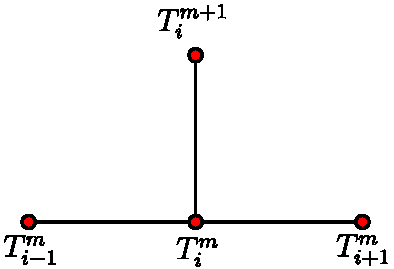
\includegraphics[width=0.35\columnwidth]{Stencils_FiniteDifferences/FTCS.pdf}
    \caption{Stencil for the Forward Time, Central Space finite difference method.}
    \label{fig:StencilFTCS}
\end{figure}

The stencil of this method can be found in figure \ref{fig:StencilFTCS}. This is considered an explicit method, as it calculates the state of the system at a later time from the state of the system at the current time. 

Introducing these approximations in equation \ref{eq:SimpleHeating}:

\begin{equation}
    \frac{T^{m+1}_i - T^m_i}{\Delta t} = H^m_i - A_i^m \left((T_i^m )^4 - (T_0)^4\right) +\alpha_i^m    \frac{T^{m}_{i-1}-2T^m_{i}+T^m_{i+1}}{\Delta x^2}
\end{equation}

After a little bit of algebra, this equation can be written in a matrix form.

$$
\begin{bmatrix}
         1 & 0 & 0 & 0 & 0 & 0 \\
         r^m_1 & \left(1-2r^m_1\right) & r^m_1 & 0 & 0 & 0 \\ 
         0 & r & \left(1-2r^m_1\right) & r^m_1 & 0 & 0 \\ 
         0 & 0 & \ddots & \ddots & \ddots & 0 \\
         0 & 0 & 0 & r^m_1 & \left(1-2r^m_1\right) & r^m_1 \\
         0 & 0 & 0 & 0 & 0 & 1 
     \end{bmatrix}
\begin{bmatrix}
         T^m_0  \\
         T^m_1 \\ 
         T^m_2  \\ 
         \vdots \\
         T^m_{N-1} \\
         T^m_N 
     \end{bmatrix}
     =
     \begin{bmatrix}
         T^{m+1}_0 + g(T^m_0) \\
         T^{m+1}_1 + g(T^m_1)\\ 
         T^{m+1}_2 + g(T^m_2)\\ 
         \vdots\\ 
         T^{m+1}_{N-1} + g(T^m_{N-1})\\
         T^{m+1}_{N} + g(T^m_{N}) 
     \end{bmatrix}
$$

With $r^m_i = \alpha^m_i \cdot \Delta t/ \Delta x^2$. And with g(T) including all the non-linear terms of the equation. In a more simplified way: 

\begin{equation}
    D_{FTCS}\cdot T^{m} = T^{m+1}+g(T^m)
\end{equation}

This is a relatively simple method to implement, as the values of $T_i^{m+1}$ can be updated independently of each other. However, the FTCS method can yield unstable solutions that can oscillate and grow if $\Delta t$ is too large. A stable solution with FTCS scheme is only obtained if: 

\begin{equation}
    r = \alpha\cdot \frac{\Delta t}{\Delta x} < \frac{1}{2}
    \label{eq:rstab}
\end{equation}

See \parencite[][]{ref:proveR1} and \parencite[][]{ref:proveR2} for a proof that equation \ref{eq:rstab} gives the stability condition for FTCS. 

\subsection{Backwards in Time, Centered Space (BTCS)}

In this case, a backward in time difference is used to approximate the time derivative while a central space scheme is used for the spatial derivative: 

\begin{equation}
    \left. \frac{\partial T}{\partial t} \right|_{t^{m+1},x_i} = \frac{T^m_i - T^{m-1}_i}{\Delta t}+\mathcal{O}(\Delta t)
\end{equation}

As in the previous case, the full equation can be represented in a matrix form: 

$$
\begin{bmatrix}
         b_0 & c_0 & 0 & 0 & 0 & 0 \\
         a_1 & b_1 & c_1 & 0 & 0 & 0 \\ 
         0 & a_2 & b_2 & c_2 & 0 \\ 
         0 & 0 & \ddots & \ddots & \ddots & 0 \\
         0 & 0 & 0 & a_{N-1} & b_{N-1} & c_{N-1} \\
         0 & 0 & 0 & 0 & a_N & b_N 
     \end{bmatrix}
\begin{bmatrix}
         T^m_0  \\
         T^m_1 \\ 
         T^m_2  \\ 
         \vdots \\
         T^m_{N-1} \\
         T^m_N 
     \end{bmatrix}
     =
     \begin{bmatrix}
         d_0 + g(T^m_0) \\
         d_1 + g(T^m_1)\\ 
         d_2 + g(T^m_2)\\ 
         \vdots\\ 
         d_{N-1} + g(T^m_{N-1})\\
         d_{N} + g(T^m_{N}) 
     \end{bmatrix}
$$

Where the coefficients are:

\begin{equation}
    \begin{gathered}
        a_i = -r^m_{i-1} \\
    b_i = 1 + 2r^m_{i}\\
    c_i = - r^m_{i+1} \\
    d_i = T^{m-1}_i + g(T_i^m)
    \end{gathered}
\end{equation}

Figure \ref{fig:StensilBTCS} shows the stencil representation of this method. In this case, we are dealing with an implicit method. To find the temperature in the time step m one must solve an equation involving both the current state of the system (m) and the previous state (m-1). 

\begin{figure}[h]
    \centering
    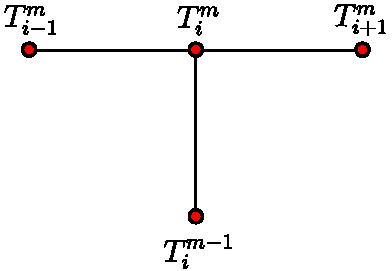
\includegraphics[width=0.35\columnwidth]{Stencils_FiniteDifferences/BTCS.pdf}
    \caption{Stencil for the Backwards in time, Central in space finite difference method.}
    \label{fig:StensilBTCS}
\end{figure}

\subsection{Crank-Nicolson}

To improve the temporal truncation error, the Crank-Nicolson scheme approximates the spatial derivative by the average of the central difference scheme, evaluated in the current (m) and the previous (m-1) time steps: 

\begin{equation}
    \frac{T^m_i - T^m_i}{\Delta t} = g(T^m_i) + \frac{\alpha^m_i}{2}\left[ 
          \frac{T^m_{i-1}- 2 T^m_i + T_{i+1}^m}{\Delta x^2} + \frac{T^{m-1}_{i-1}-2T^{m-1}_i+T_{i+1}^{m-1}}{\Delta x^2}
    \right] 
\end{equation}

This method is implicit, like the BTCS method. However, it accomplishes a truncation error $\mathcal{O}(\Delta t^2)$ without overcomplicating the implementation. The matrix representation is the same as in the BTCS case, but with the following coefficients:

\begin{equation}
    \begin{gathered}
        a_i = -r^m_{i-1}/2 \\
        b_i = 1 + r^m_{i}\\
        c_i = - r^m_{i+1}/2 \\
        d_i = a_i T_{i-1}^{m-1} + (1 + a_i + c_i) T^{m-1}_{i} + c_i T_{i+1}^{m-1} + g(T_i^m)
    \end{gathered}
\end{equation}

The stencils representation of this method is shown in Figure \ref{fig:StencilCrNic}.

\begin{figure}[h]
    \centering
    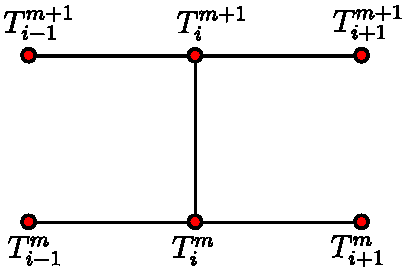
\includegraphics[width=0.35\columnwidth]{Stencils_FiniteDifferences/CrkNic.pdf}
    \caption{Stencil for the Crank-Nicolson finite difference method.}
    \label{fig:StencilCrNic}
\end{figure}

\section{Initial and Boundary Conditions}

Due to the time dependent part of our equation, we need an initial condition. In this case, this refers to the temperature of the system at time $t^0$. Unless specified otherwise, a constant temperature $T_{i,j}^0 = 300 (K)$ will be considered.

At each time step, because of the spatial dependence of the equation, some boundary conditions need to be specified. Here the so-called Dirichlet boundary conditions are considered. For the one-dimensional case, these conditions can be written as follows: 

\begin{equation}
    \begin{cases}
      T(0,t) = 300 \mspace{30mu} (K) \\
      T(L,t) = 300 \mspace{30mu} (K) 
    \end{cases}
\end{equation}

Where L refers to the length of the one-dimensional rod. In the 2D case, these conditions would indicate that all the borders of the foil are in contact with a thermal sink at 300 (K). 

\section{The Non-Linear Problem}

In the previous sections, g(T) was described as the non-linear term. The explicit expression is: 

\begin{equation}
    g(T) = \frac{N(x,t)}{V\cdot Cp(T)\cdot \rho(T)}\frac{dE}{dz} - \frac{S\cdot \sigma_{SB}\epsilon(T)\cdot \left( T(x,t)^4 - T_0^4\right)}{V\cdot Cp(T)\cdot \rho(T)}
\end{equation}

In the case with no heating and no radiative cooling, g(T) = 0. This case yields to the diffusion equation. In this scenario, the systems of equations presented in the previous section can be easily solved by techniques such as Gaussian elimination methods, LU factorization, etc. More information about those methods can be found in \parencite[][]{ref:AlvaroBook}. 

$g(T) \neq 0$ implies that now, at each time stem, one has to solve a system of non-linear equations. This is still solvable numerically, but it implies using other numerical techniques such as Newton's method for non-linear systems \parencite[][]{ref:AlvaroBook}. At every time step, one must guess an approximate solution and compute the Jacobian matrix. Which can be computationally expensive and cumbersome. 

By default, instead of considering the full equation, each term of the equation is considered separately and then added together. For equation \ref{eq:SimpleHeating} this would mean solving the following: 

\begin{equation}
    \frac{\partial \Delta T_{Ht} (x,t)}{\partial t} = H(x,t,T)
\end{equation}
\begin{equation}
    \frac{\partial \Delta T_{Rad} (x,t)}{\partial t} = A(T) \left(T(x,y)^4 - T_0^4\right)
\end{equation}
\begin{equation}
    \frac{\partial \Delta T_{Con}}{\partial t} = \alpha(T)\frac{\partial^2 T(x,t)}{\partial x^2}
\end{equation}

The total temperature variation is then calculated as: 

\begin{equation}
    \Delta T_{tot} = \Delta T_{Ht} - \Delta T_{Rd} - \Delta T_{Con}
\end{equation}


\section{The two-dimensional problem}

In the previous section, we developed the equations for the one-dimensional case due to the simpler notation. The biggest difference in the two-dimensional case is the conduction term on the heat equation. Each point in space is now connected to four other points, that is, there is conduction along four rods. Figure \ref{fig:1Dvs2D} shows a schematic representation of the differences between nodal connections in a 1D and 2D case.  

\begin{figure}[h]
    \centering
    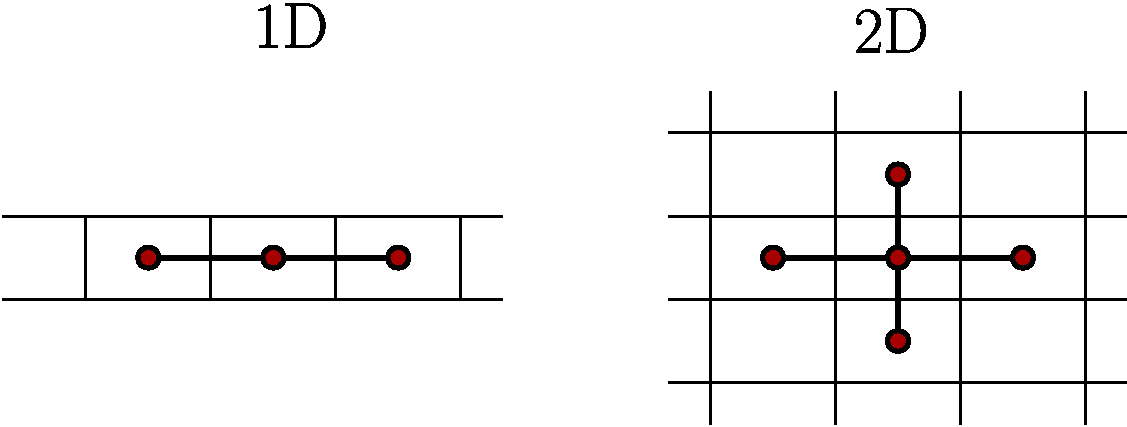
\includegraphics[width=0.60\columnwidth]{1D_vs_2D_cond/1Dvs2F.pdf}
    \caption{Schematical comparison between 1D (left) and 2D (right) nodal connection.}
    \label{fig:1Dvs2D}
\end{figure}

For the two-dimensional case, a five-point finite difference formulation is used \parencite[][]{ref:FiniteDifference}. Taking the simplified case of the 2D diffusion equation: 

\begin{equation}
    \frac{\partial T(t,x,y)}{\partial t} = \alpha (T) \left(\frac{\partial^2 T}{\partial x^2}+\frac{\partial ^2 T}{\partial y^2}\right)
\end{equation}

One could write the FTCS formulation as follows: 

\begin{equation}
    \frac{T_{i,j}^{m+1} - T_{i,j}^{m}}{\Delta t} = \alpha(T_{i,j}^{m}) \left( \frac{T_{i-1,j}^{m} -2T_{i,j}^{m}+T_{i+1,j}^{m}}{\Delta x^2} +  \frac{T_{i,j-1}^{m}-2T_{i,j}^{m}+T_{i,j+1}^{m}}{\Delta y^2} \right)
\end{equation}

Similarly, this could be applied to the BTCS and Crank-Nicolson formulations. The same procedure to transform this into a system of equations can also be followed. 

\section{Importance of Cooling Effects}

The most accurate simulation is obtained when all the cooling mechanisms indicated in equation \ref{eq:HeatBalance} are considered. However, if simulation speed is what matters, a fuster simulation can be run by ignoring certain cooling mechanisms. Particularly, conduction cooling is the most time-consuming one. Figure \ref{fig:CoolingComparison} shows how much each cooling mechanism contributes to the total cooling as a function of the temperature. This figure was calculated for a $30 \mu m$ Graphite wire. It might differ slightly for different materials and geometries. 

From this figure, one can observe how radiation cooling is the predominant mechanism throughout the biggest temperature range. Conduction cooling plays a very important role at lower temperatures while thermionic and sublimation cooling are important only at very high temperatures. 

If there is some a-priory knowledge of the expected temperature range, or simply a fast upper limit of the maximum temperature is needed, various cooling processes can be deliberately eliminated for speed purposes.

\begin{figure}[h]
    \centering
    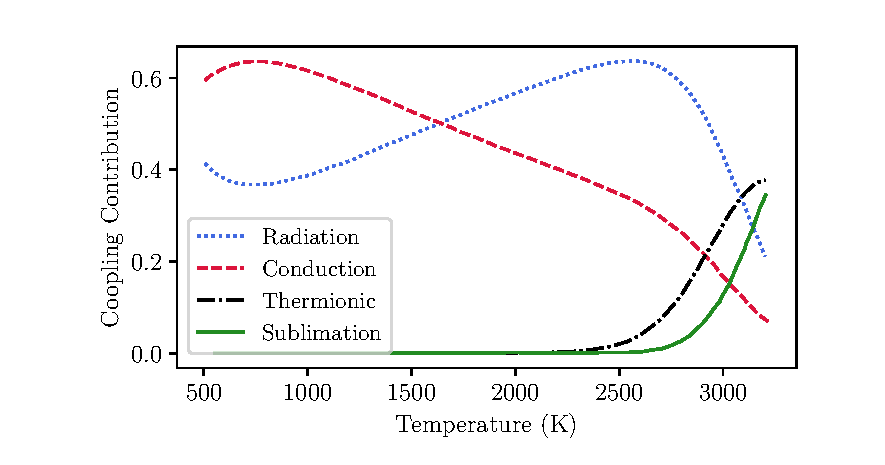
\includegraphics[width=0.60\columnwidth]{PlotCoolingImportancfe/CoolingImpo.pdf}
    \caption{Relative importance of the different cooling mechanisms as a function of the temperature.}
    \label{fig:CoolingComparison}
\end{figure}

\section{PyTT}

The simulation program was implemented using Python 3.6.9. The latest version of the code can be found at \parencite[][]{ref:GitAra}. As aforementioned, the main objective of this code is to quickly obtain an estimation of the maximum temperature reached by thin target detectors when interacting with the beam of particles. Additionally, the code also needed to be easy to use by people who aren't particularly familiar with python or numerical techniques.

Figure \ref{fig:UserFriendly} shows the GUI of the implemented program. The program can also be run directly, without the GUI which allows for easy parallelization. The implementation of the code and its usage will not be discussed in this document. Just the main description of its functionalities will be given. 

\begin{figure}[h]
    \centering
    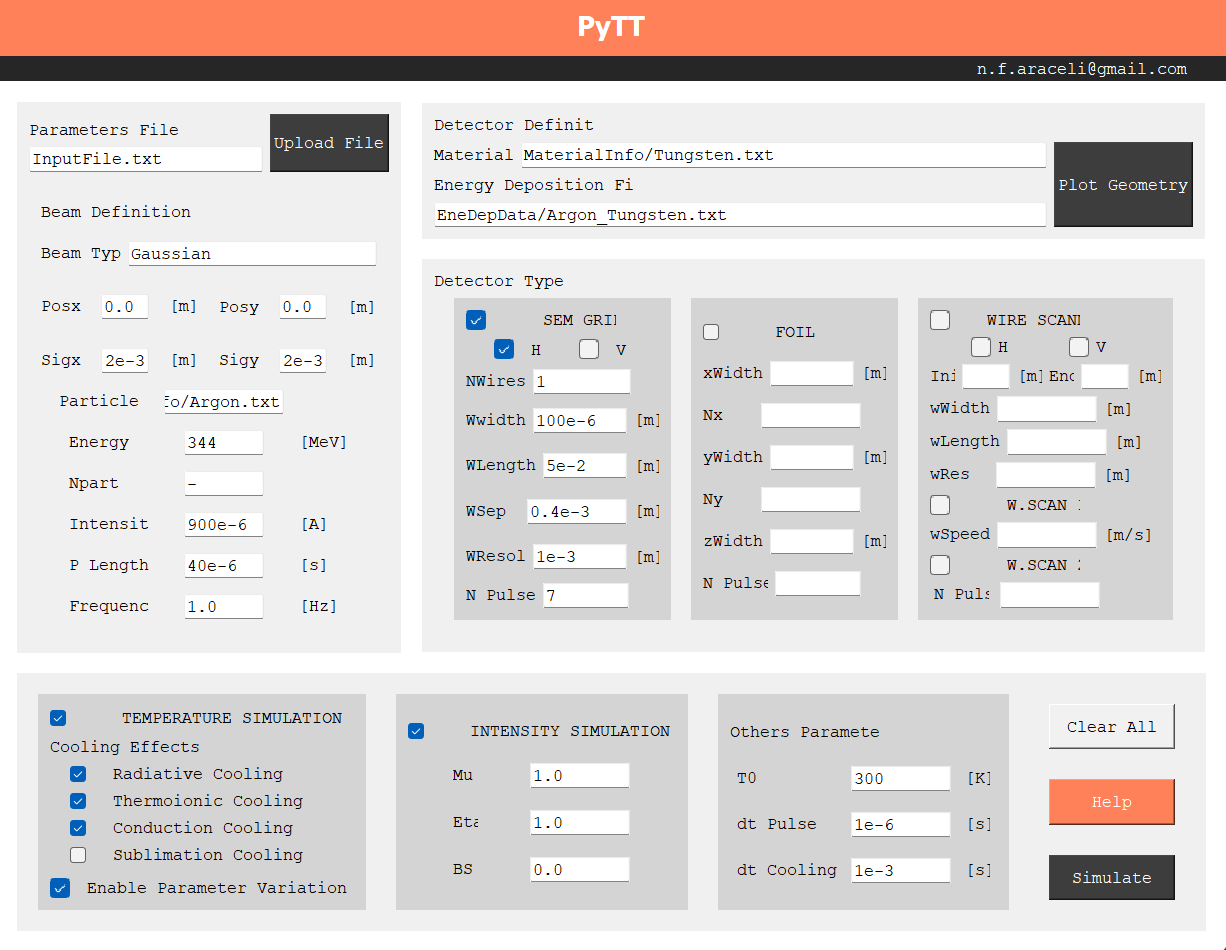
\includegraphics[width=0.9\columnwidth]{PyTT_GUI/PyTTScreanshot.png}
    \caption{Graphical User-Friendly interface of PyTT code.}
    \label{fig:UserFriendly}
\end{figure}

\begin{enumerate}
    \item Variety of Beam Conditions: To simulate a variety of cases, the program allows the user to choose several beam parameters. For example, the particle or ion type and energy, the spatial and temporal distribution, and the repetition frequency of the particle beam. 
    \item Variety of Detector Materials: The material of the detector can be chosen freely, by either selecting one of the already given materials or by easily creating one's own. 
    \item Type of thin target detectors: The program can simulate SEM grid detectors, Thin foils and Wire scanners. For the wire scanners, both fast and slow wire scanners can be considered. 
    \item Choosable simulation Parameters:  Several simulation parameters (Such as space-time discretization parameters, simulation length, thermal effects, parameter temperature dependence, etc.) Can be easily selected at the user's convenience. 
    \item Intensity Simulation: The program includes an intensity simulation module that includes the model explained in chapter \ref{ch:CurrentModeling}. This calculates the current generation in the detector during operation. 
\end{enumerate}

Results like the maximum temperature in the detector as a function of time are provided by default. Figure \ref{fig:GUIResults} shows an example of the simulated output. However, using the output files produced by the simulation, some additional results can be attained. These can include, spatial thermal distributions, the relative importance of the different cooling methods, the evolution of material properties during simulation, intensity distribution, etc. 

\begin{figure}[h]
    \centering
    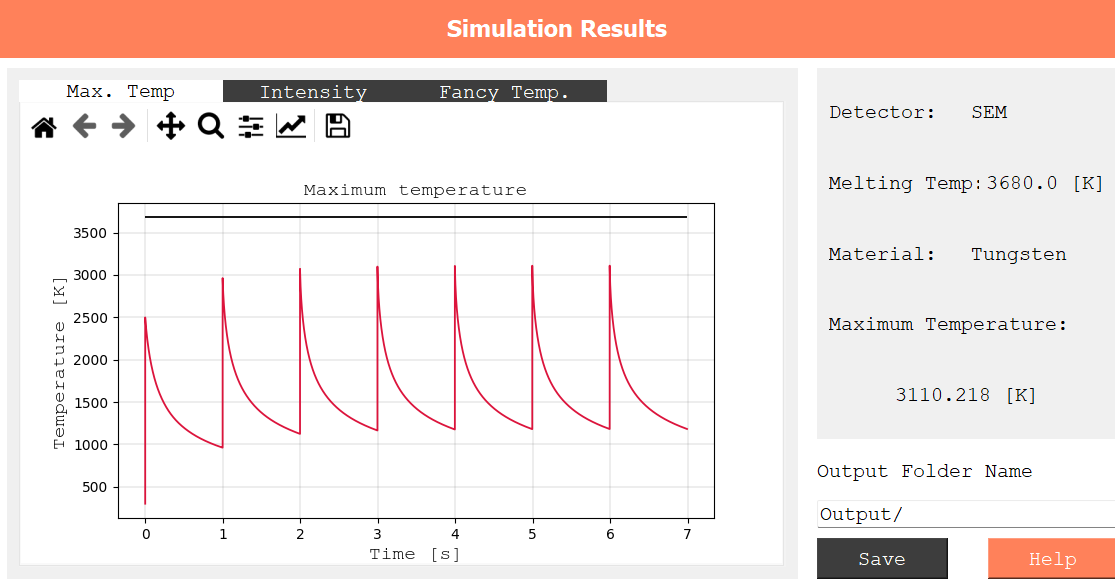
\includegraphics[width=0.9\columnwidth]{PyTT_GUI/PyTTresults.png}
    \caption{Example of output visualization GUI.}
    \label{fig:GUIResults}
\end{figure}

The program has been optimized for it to be used by the python interface. However, it can also be launched by a stand-alone executable for windows systems. A more detailed description of how to use the code can be found in the user manual, accessible through the help button in the GUI, or directly in the HelpFolder.

\section{Model uncertainties}
\label{sec:ModelUnc}

As with all models, the approximations done along the way induce uncertainties in the final results. In section \ref{sec:FD} we talked about the order of truncation errors. We saw how errors were related to the selection of space-time discretization sizes. In this section, we will talk about other sources of error that have proven to be more significant than the numerically induced uncertainties. 

The simulation results highly depend on our knowledge of the simulation case. That is, the better one is able to describe the experimental situation, the more accurate the simulated results. However, a lot of different parameters are involved in this description. To simplify the study one can divide these parameters into two categories: Beam Parameters and Material Properties. 

\subsection{Beam Parameter Uncertainties.}

These parameters are the ones used to describe the spatial and temporal distribution of the beam of particles. If we take as an example the case of a Gaussian beam, those parameters would be: beam size ($\sigma_x , \sigma_y$), beam position, Intensity, pulse length, repetition rate, etc. 

Figure \ref{fig:BeamParUnc} shows how uncertainties in the beam parameters affect the final temperature simulated results. To clarify, to calculate these values, a case was considered to be the average, or correct solution. All the parameters were varied independently up to a $\pm 30\%$ of their value (Parameter Rel. Error)  and the relative error of the simulation was calculated in each case with respect to the average solution. 

From this figure, we can observe that uncertainties in the beam Intensity and pulse length give an almost identical uncertainty response, which increases linearly with the parameter uncertainty. Uncertainties in the beam size, greatly affect the final uncertainties in the maximum simulated temperatures. First, notice the non-symmetry of the results, smaller beam sizes greatly affect the final results. Larger beam sizes induce smaller uncertainties. 

\begin{figure}[h]
    \centering
    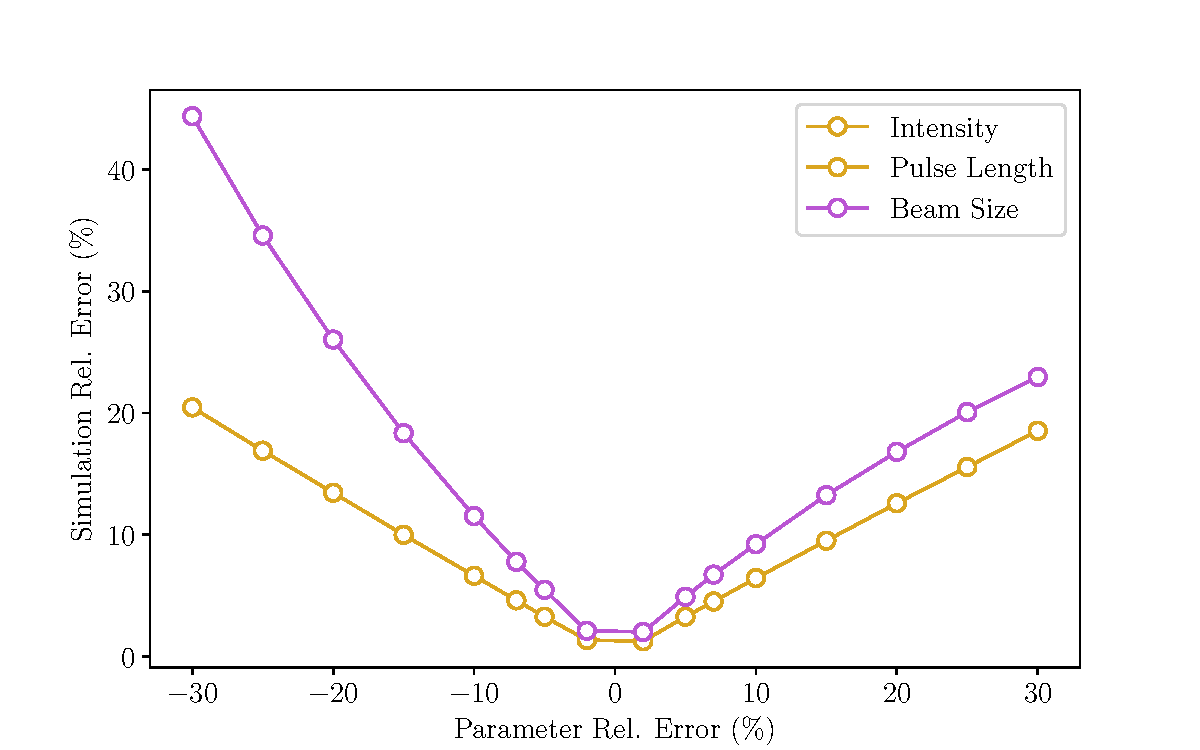
\includegraphics[width=0.7\columnwidth]{BeamParameterUncertainty/BeamParUnc.pdf}
    \caption{Effects of beam parameter uncertainties on maximum temperature simulation results.}
    \label{fig:BeamParUnc}
\end{figure}

It is difficult to give a specific value of the Beam parameters uncertainty, as it is very much dependent on the simulation case. If the range of confidence of the simulation studies is necessary for a certain application a proper study of the Beam parameter uncertainties should be carried out. 

\subsection{Material Parameter Uncertainties.}

Material parameters are all those material properties that are necessary for the simulation. These properties are compiled in Table \ref{tab:MaterialProp}. In most cases, the values of these parameters are well known and can be found in the literature. A very good reference for metallic and non-metallic solids is \parencite[][]{ref:MatProperties}.  

\begin{table}[h]
    \centering
    \begin{tabular}{ccc}
    \hline
    \textbf{Property} & \textbf{Abbreviation} & \textbf{Units} \\ \hline
    Atomic Number     & Z                     &                \\
    Atopic Mass       & A                     & amu            \\
    Density           & rho                   & g/cm3          \\
    Melting Point     & Mp                    & K              \\
    Work Funktion     & phi                   & eV             \\
    Emissivity        & eps                   &                \\
    Specific Heat     & Cp                    & J/gK           \\
    Conductivity      & k                     & W/mK           \\ \hline
    \end{tabular}
    \caption{Material parameters necessary for thermal simulations.}
    \label{tab:MaterialProp}
    \end{table}

Similarly to the beam parameter case, figure  \ref{fig:MatPar} shows the effects uncertainties in the different material parameters have on the final maximum temperature uncertainties. In this case, one can observe how the parameter that induces the highest uncertainty is the specific heat (Cp). How big are the uncertainties is very much dependent on the material. To give a numerical example of typical uncertainty values we studied the Graphite and the tungsten case. 

\begin{figure}[h]
    \centering
    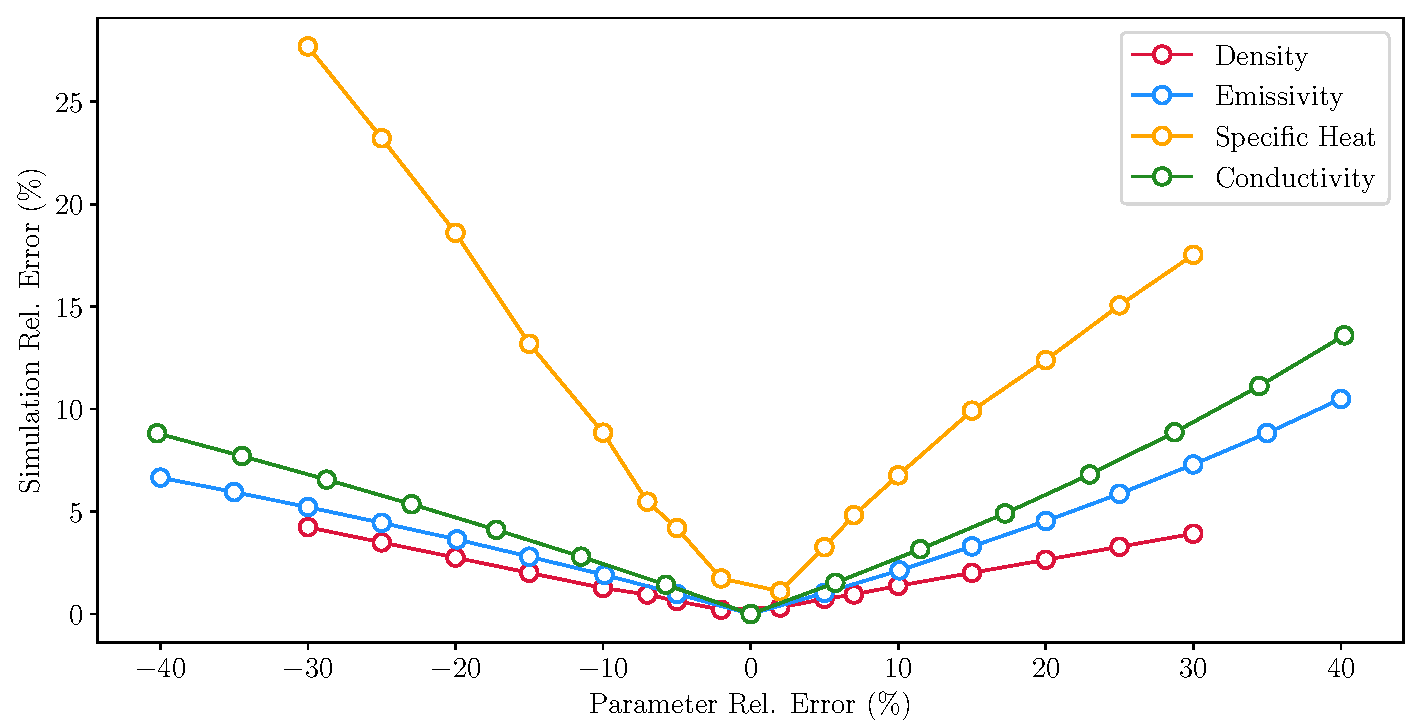
\includegraphics[width=0.7\columnwidth]{MaterialParameterUncertainty/MatParUnc.pdf}
    \caption{Effects of material property uncertainties on maximum temperature results.}
    \label{fig:MatPar}
\end{figure}

Figure \ref{fig:MatPropUnc} shows the uncertainties for specific heat, emissivity and thermal conductivity
parameters for Tungsten and Graphite. In this case, the uncertainties for the other parameters were negligible. This figure was obtained by collecting the values of the material properties reported by different sources. The central points on the boxes represent the average property value, while the limits of the colored boxes represent the RMS. The error bars represent the maximum and minimum discrepancies found with respect to the average value. 

\begin{figure}[h]
    \centering
    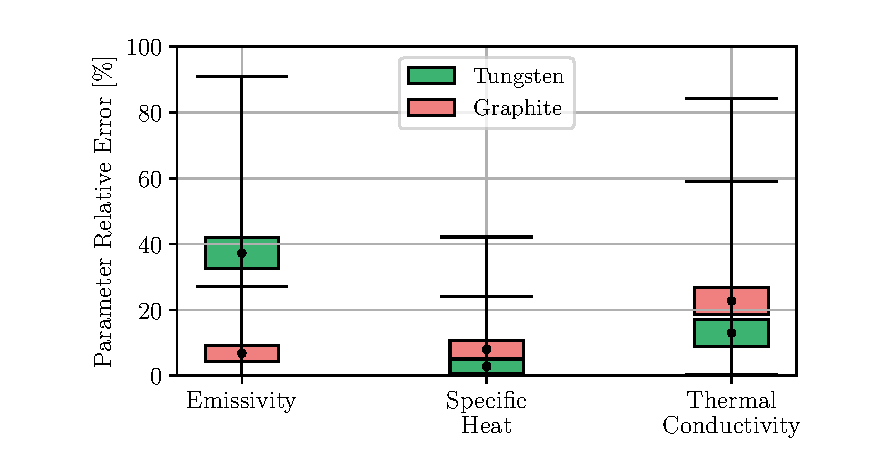
\includegraphics[width=0.7\columnwidth]{PlotTungstenGraphiteUncertainty/GraphTungsUnc.pdf}
    \caption{Material property uncertainties for Graphite and Tungsten. }
    \label{fig:MatPropUnc}
\end{figure}

Uncertainties of the Specific heat are quite small ($2.83 \% $) for both graphite and tungsten. In the case of graphite, values for the emissivity seem to be quite well known ( $ 6.75\%$). Contrarily, a much higher uncertainty was found in the case of its thermal conductivity ( $ 22.71\%$). In the case of tungsten, we find the opposite situation, different sources seem to agree on the value of the thermal conductivity ($13.0\%$ ), however, big uncertainties are found in the emissivity case ($43.26 \%$). 

This big uncertainty in the tungsten emissivity led to an in-depth investigation. To reduce the overall uncertainty of the simulations for tungsten detectors. These experimental measurements and the obtained results will be covered in Chapter \ref{ch:EmissivityMeas}.

\section{Aplications: Beam Power Limit Calculations}

Determining beam power limits means determining beam conditions that could potentially damage the detectors. To do that, the PyTT program was used to simulate the maximum temperatures reached by the detectors for the different expected beam conditions at their location. If the maximum temperature reached was above the safe limit, those beam conditions were considered to be harmful to the detectors. 

\subsection{SEM grid and Slow Wire Stanner at Linac4}

For Linac4, the beam conditions under study were: Beam Intensity ($I_{beam}$), beam pulse length ($\Delta t$) and beam size ($\sigma_x , \sigma_y$). Figure \ref{fig:DetLoc} shows a schematic representation of Linac4, with the different detectors location. The detectors in the L4L, L4D and L4C lines are made of graphite wires ($33 \mu m$). The rest of the wire scanner detectors are also graphite wires, whereas the SEM grid detectors are gold-coated tungsten wires ($40 \mu m$). Table \ref{tab:beamprop} summarizes the range of the beam properties expected at the Linac4 accelerator.

For each detector, a set of dedicated simulations covering the whole parameter range were performed with the PyTT program. A maximum temperature of 1400K was taken as a safe maximum temperature limit. This limit is probably very conservative, as most of the detectors could easily handle up to 3000 K. However, due to the wire-gluing problem suffered in SEM grid detectors, a much lower temperature limit was established. 

\begin{figure}[h]
    \centering
    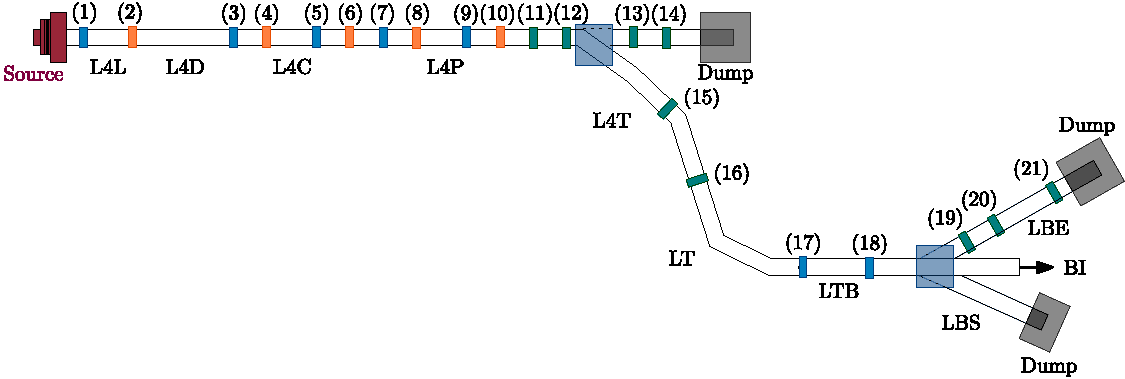
\includegraphics[width=1.0\columnwidth]{Figure_Linac4Instrumetnation/DetecPos.pdf}
    \caption{Schematic representation of Linac4 with SEM grid (blue boxes), wire scanner (orange boxes) locations. Green boxes indicate locations where both, sem grid and wire scanners are installed.}
    \label{fig:DetLoc}
\end{figure}


\begin{table}[h]
    \centering
    \begin{tabular}{cccc}
    \hline
    Property                          & Min & Max & Units   \\ \hline
    Intensity ($I_{beam}$)            & 10  & 25  & mA      \\
    Pulse Length ($\Delta t$)         & 50  & 400 & $\mu s$ \\
    Beam Size ($\sigma_x , \sigma_y$) & 0.5 & 3.0 & mm      \\ \hline
    \end{tabular}
    \caption{Range of beam properties expected at Linac4 accelerator.}
    \label{tab:beamprop}
\end{table}

Figure \ref{fig:EnerCompa} shows an example of the power limits calculated for a detector in L4C line (Detector 5) and a detector at the L4T line (Detector 12). Each square represents the maximum temperature reached by a simulation with the beam pulse length indicated on the X axis, and the beam intensity indicated on the Y axis. The beam size in both cases was $\sigma_x = \sigma_y = 2.0 (mm)$ . 

In both cases, we can observe that beam pulse lengths smaller than 200 $\mu s$ are very safe. Neither detector was getting close to the set temperature limit. One interesting observation is in this case the difference in the results between the detector located at the L4C line and the one located at the L4T line. The only difference between the detectors is the energy deposition in the material. At higher energies, the energy deposition is smaller, so the maximum temperatures reached by the detector are smaller than the equivalent conditions at lower energies. 

\begin{figure}[h]
    \centering
    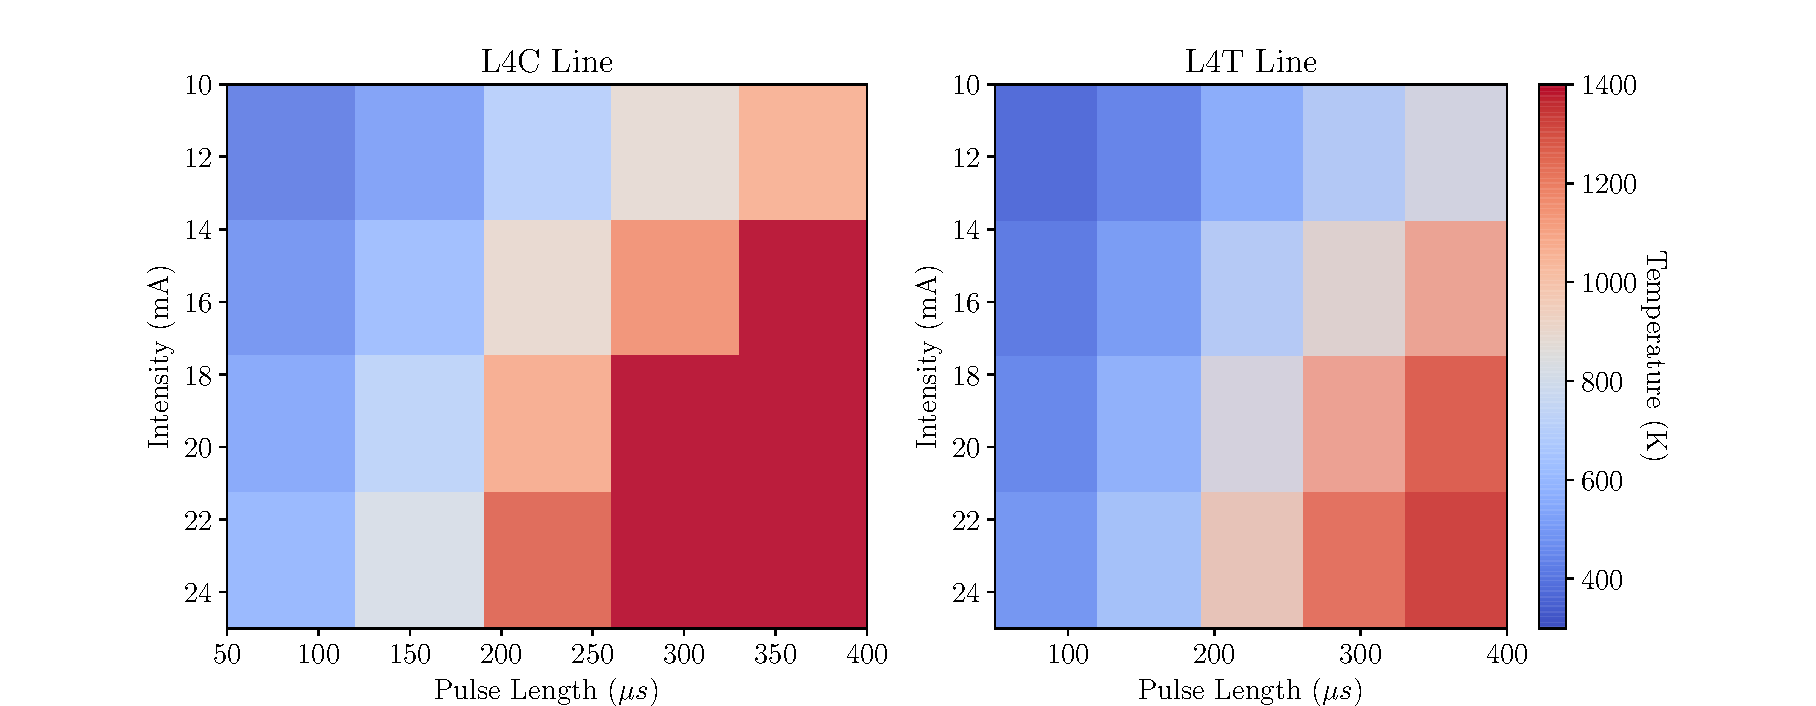
\includegraphics[width=1.0\columnwidth]{Figure_ThermalLimitsSquares/EnergyCompa.pdf}
    \caption{Power limit calculations for a detector at L4C (Left) and a detector at L4T (right) lines. The beam size in both cases was $\sigma_x = \sigma_y = 2.0 (mm)$.}
    \label{fig:EnerCompa}
\end{figure}

Figure \ref{fig:SigmaComparison} shows a similar set of results, but this time, both detectors were placed at locations where the particle energy was already 160 MeV. The difference between the right plot and the left plot is the beam size. The left hand side figure pictures a small beam size ($\sigma_x = 0.8$ (mm), $\sigma_y = 2.0$ (mm)). The right-hand side figure pictures a larger beam size ($\sigma_x = 1.2 (mm)$). From this figure, we can observe how small beam sizes result in much more critical thermal conditions. 

In general, one should be very careful measuring small beam sizes at low energy ranges. An overall power limit for the Linac4 accelerator was established. Beam conditions were considered to be dangerous if the beam size was smaller than 1 $(mm)$ and the beam pulse length was longer than $100 ()\mu s)$. An interlock system for SEM grids and wire scanners was established at Linac4 based on these results. 

\begin{figure}[h]
    \centering
    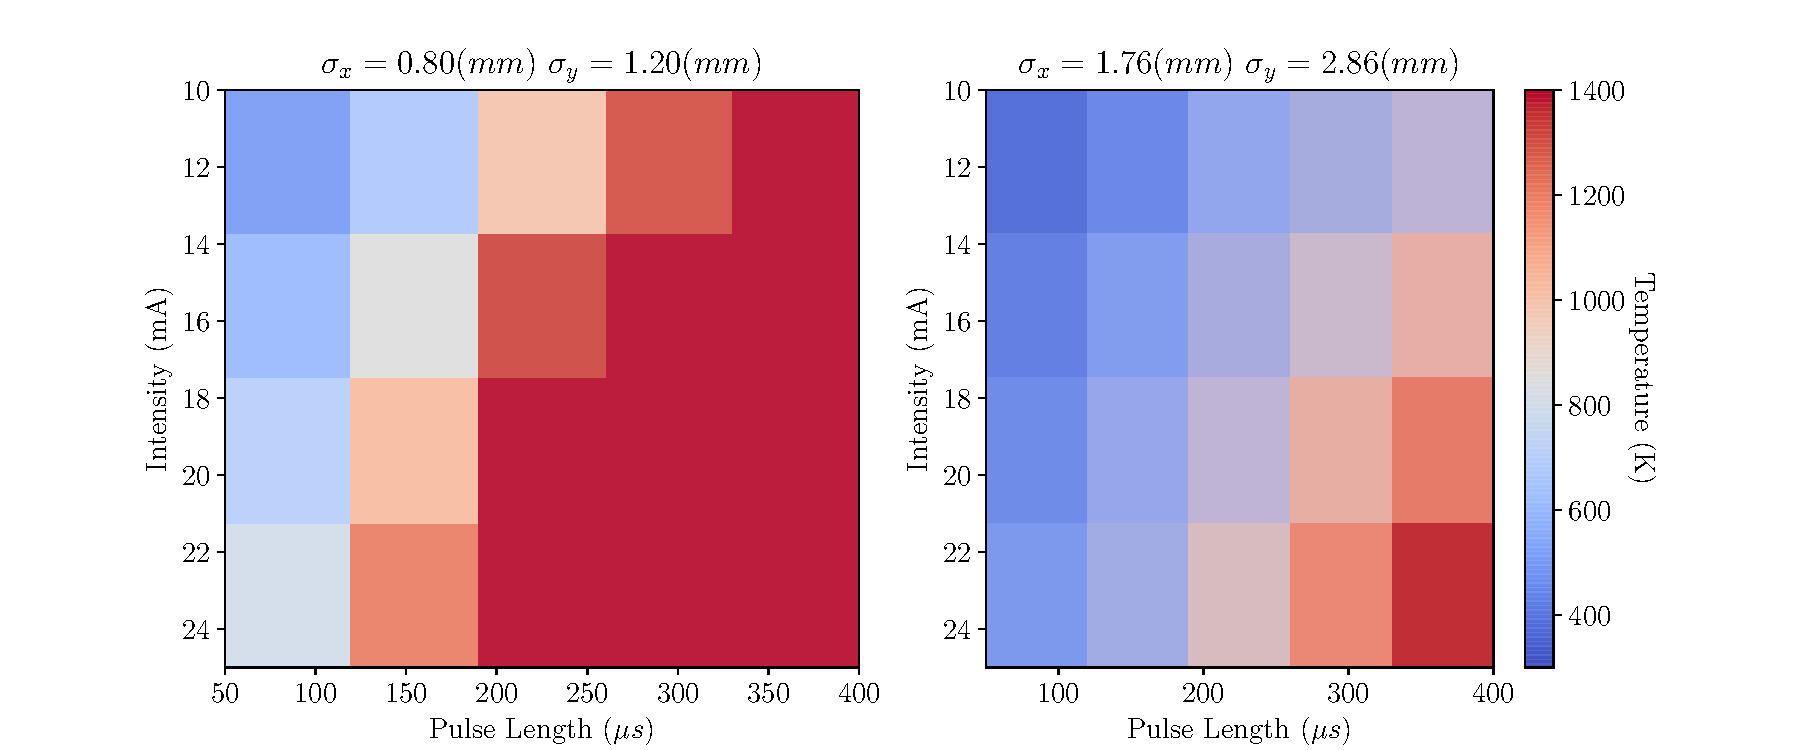
\includegraphics[width=1.0\columnwidth]{Figure_ThermalLimitsSquares/SigmaCompa.pdf}
    \caption{Power limit calculations for a detector at 160 MeV beam energies.}
    \label{fig:SigmaComparison}
\end{figure}

\subsection{Fast Wire Scanners at SPS}

A new generation of beam wire scanners has been developed at CERN, in the framework of the LIU project \parencite[][]{ref:WireScanJose}. In the SPS, 4 new wire scanner systems were installed, for horizontal and vertical beam size measurements. In this case, the relevant parameters under study were: beam emittance (at injection and extraction), the number of protons per bunch (from $10^9$ to $10^{11}$), the maximum number of bunches (from 1 to 288) and wire scanner velocity (form 1 m/s to 20 m/s). 

For the SPS energies ( 26 GeV at injection and 450 GeV at extraction ) differences in energy deposition are not as important as in the Linac4 case. Beam sizes are still a very important parameter to consider. In the SPS, the beam size is usually described in terms of beam emittance. One can easily convert from one to the other with the following relation: 

\begin{equation}
    \sigma = \sqrt{\frac{\epsilon_{norm}}{\gamma_{rel} \cdot \beta_{rel}} \cdot \beta(s)}
\end{equation}

Where $\epsilon_{norm}$ refers to the normalized emittance and $\beta_{rel}$, $\gamma_{rel}$ are the relativistic parameters. $\beta(s)$ is the courant-Snyder parameter at the position s. Because the beam size decreases as the relativistic parameters increase, smaller beam sizes are found in the extraction case. 

Figure \ref{fig:WireScanner1} shows the evolution of the maximum temperature reached by a 33 $\mu m$, graphite, fast wire scanner for a different number of particles per bunch. In this figure, the wire scanner speed was set constant to 1 m/s, and the total number of bunches was always 288.  The figure on the left is for injection energies (26 MeV) and the one on the right is for extraction energies (450 MeV). In both cases, the higher the number of particles per pulse the higher the temperature reached by the detector. 

In these figures, we can also see the decrease of the beam size with the energy, as the temperature increase happens in a much narrower period during extraction energies. 

\begin{figure}[h]
    \centering
    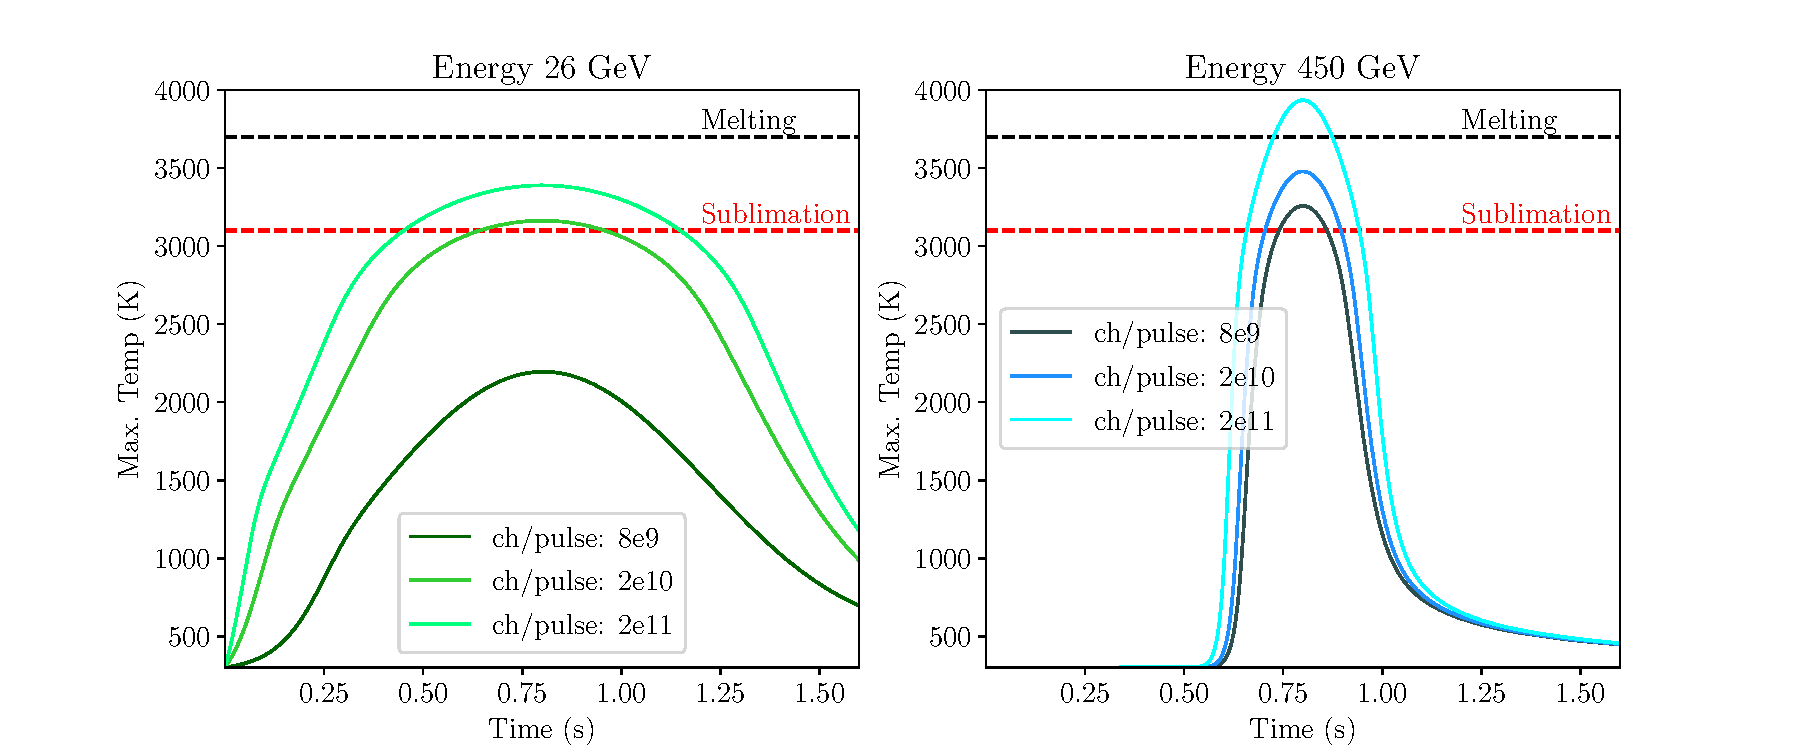
\includegraphics[width=1.0\columnwidth]{WireScanner_Limits/WireLim1.pdf}
    \caption{Comparison of maximum fast wire scanner temperatures reached for different beam conditions. Left: Injection energy. Right: Extraction energy.}
    \label{fig:WireScanner1}
\end{figure}

The wire velocity is also a very important factor to consider. The slower the wire velocity the longer time it will spend in the central area of the beam, and thus the higher the maximum temperature reached. Increasing the wire speed is beneficial in terms of thermal limitations. However, as a tradeoff, we have the measurement resolution. Because the wire scanner in the SPS is much slower than the bunches being accelerated (revolution period $t_{rev} = 2.4\cdot 10^{-5} s$). The number of points per sigma taken by a fast wire scanner can be calculated as: 

\begin{equation}
    n_{points} = \frac{\sigma}{v_{w}\cdot T_{rev}}
\end{equation}

For a beam size of 1 mm, a maximum speed of 10 m/s can be used. Otherwise, the measurements would not have enough resolution. 

The wire damage can be associated with the density of charges traversing the wire \parencite[][]{ref:Msapinski}:

\begin{equation}
     n_{ch} = \frac{N_{ch} \cdot d_{w}}{v_{w} \cdot t_{rev} \cdot \sigma}
\end{equation}

Where $N_{ch}$ is the total number of particles, understood as the number of particles per pulse times the number of pulses. $d_w$ is the wire diameter and $v_w$ is the wire velocity. As a limiting scenario, we could consider the case of a 33 $\mu m$ Graphite wire, with a speed of 1 m/x and measuring a beam size $\sigma_x = \sigma_y = 0.3$ (mm).   In this case the density of particles $n_{ch} = 2.5\cdot 10^{12}$. Beam and wire conditions yielding a charge density higher than this number, are considered to be potentially harmful.

This number is consistent with the experiments performed by M. Sapnski \parencite[][]{ref:Msapinski}. This value is used in the SPS accelerator as a safety limit. Table \ref{tab:MaxNturns} shows an example of how this safety value was used to calculate the maximum number of allowed turns for different wire scanners and beam conditions. At CERN SPS, the maximum number of injected turns can go up to 288. From this table, we can observe that only at injection energies this number of bunches can be measured. 

% Please add the following required packages to your document preamble:
% \usepackage{multirow}
\begin{table}[h]
    \centering
    \begin{tabular}{cclccccc}
    \hline
    \multirow{2}{*}{\begin{tabular}[c]{@{}c@{}}Energy \\ (GeV)\end{tabular}} & \multicolumn{2}{c}{Beam Size (mm)} & \multicolumn{5}{c}{Wire Velocity (m/s)} \\ \cline{2-8}    & $\sigma_x$               & $\sigma_y$              & 1     & 6      & 10    & 15    & 20     \\ \hline
    \multirow{2}{*}{25}                                                      & 3.03             & 2.10            & 54    & 323    & 538   & 807   & 1080   \\
     & 2.0              & 1.38            & 35    & 213    & 350   & 531   & 708    \\ \hline
    \multirow{2}{*}{450}   & 0.72             & 0.50            & 12    & 74     & 129   & 194   & 258    \\    & 0.47             & 0.33            & 8     & 51     & 85    & 127   & 170    \\ \hline
    \end{tabular}
    \caption{Maximum allowed number of beam bunches for different beam conditions. The number of charges per bunch was $1.5 \cdot 10^{11}$ ch/bunch. }
    \label{tab:MaxNturns}
\end{table}